\documentclass[9pt]{beamer}
\usepackage{beamerthemesplit} % new 
\usepackage{tcolorbox}
\usepackage{hyperref}
\usepackage{subfigure}
\usepackage{color}
%\usetheme{Frankfurt}
\usetheme{Madrid}
%\usetheme{Copenhagen}

%Document begins
\begin{document}
\title{Communication Complexity} 
\author{Sushovan Majhi}
\date{\today} 
%\date{April 26, 2016}
\frame{\titlepage} 

\begin{frame}
  \begin{center}
    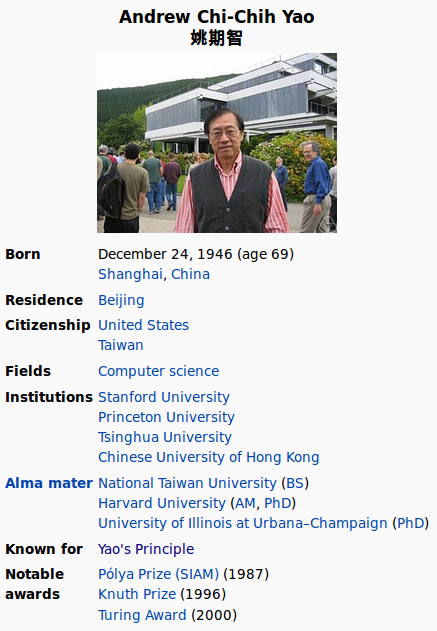
\includegraphics[scale=0.4]{yao.png}
  \end{center}
\end{frame}

\begin{frame}{Communication Everywhere}
  \begin{center}
    
\includegraphics[scale=0.2]{network.jpg}
  \end{center}
  \textcolor{red}{Communcation exists because of the limitation of resources in a 
    single system}
\end{frame}

%% \frame{\frametitle{Complexity::Basics}
%%   \begin{block}{Defining A Problem/Task}
%%     Suppose we have a problem or task$P$ e.g. soring $n$ number, 
%%     finding a hamiltonian cycle in a graph, 
%%     summing two integers, find an assignment of the variables that satisties a boolean function 
%%     etc.\\
%%     $$P(Input)=Output$$
%%   \end{block}
%%   \pause
%%   \begin{block}{Making It Rigorous}
%%     A problem can be thought of as a function 
%%     $$f:\{0,1\}^*\to\{0,1\}^*$$
%%   \end{block}
%% }

%% \frame{\frametitle{Complexity::Basics}
%%   \begin{block}{Algorithm}
%%     Methods/Protocols/Turing machines that solve the given problem $P$ or compute the corresponding 
%%     boolean function $f$ in finitely many steps for any value of the input.\\
%%   \end{block}
%%   \pause
%%   \begin{block}{}
%%     Let $\mathcal{T}(P)$ denote the sets of all algorithms that solve $P$.
%%   \end{block}
%%   \pause
%%   \begin{block}{Measure Of Complexity(Cost Of Computation)}
%%     For an $A\in\mathcal{T}(P)$, $\mu($P$)$ measure how expensive the protocol $A$ is over all 
%%     possible inputs of a fixed length $n$.\\
%%     Usually it's the time and/space used by the algorithm $A$ to solve our problem $P$.
%%   \end{block}
%% }

%% \begin{frame}{Complexity::Basics}
%%   \begin{block}{Complexity Of A Task::Lower And Upper Bounds}
%%     Complexity of the task $P$ is $$C(P)=\min_{A\in\mathcal{T}(P)}\mu(A)$$
%%     Roughly speaking, it is the complexity of the best algorithm possible for the task $P$.
%%   \end{block}
%%   \pause
%%   \begin{block}{Computer Scientists Are Lazy!}
%%     $C(P)$ is a function of $n$(input length).\\
%%     We use big-$O$, $\theta$, $\Omega$ notation to hide nasty coefficients and unnecessary lower 
%%     order terms. \\
%%   \end{block}
%%   \pause
%%   \begin{block}{Examples}
%%     If $C(P)=2015n^2 + 2016\log\log\log\log n + 2017$, we say $C(P)\in O(n^2)$.\\
%%     \pause
%%     E.g. $C(Sorting)\in O(n^2)$ \textcolor{green}{Upper bound}\\
%%     \pause
%%     $C(Sorting)\in\Omega(n\log n)$ \textcolor{red}{Lower bound}\\
%%   \end{block} 
%% \end{frame}

\begin{frame}{Setting Up The Stage}
  Given a boolean function $$f:X\times Y\to\{0,1\}$$ that both Alice and Bob want 
  to compute on an 
  input(x,y). \\
  Let's take $X=Y=\{0,1\}^n$.
  \begin{center}
    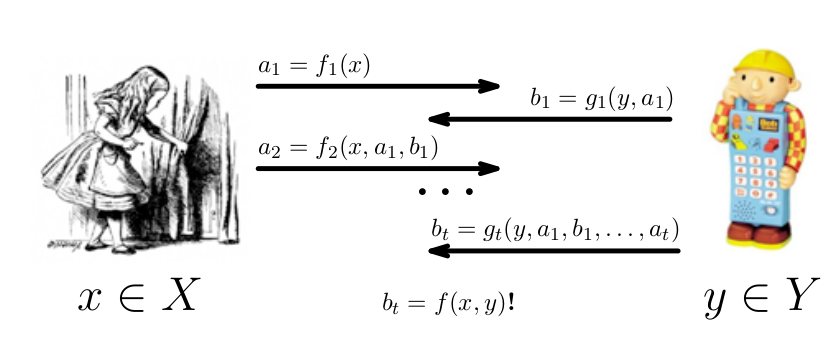
\includegraphics[scale=0.25]{alice_bob.png}
  \end{center}
  \pause
  \begin{block}{Assumptions}
    \begin{enumerate}[i)]
    \item We have a two ``party'' or "player'' communication system. 
      \pause
    \item The communication channel is completely secure and noiseless. 
      \pause
    \item The parties have \textcolor{red}{unbounded/infinte computational power}.
      \pause
    \item The number of rounds or the size of the sets $X$,$Y$ are not that 
      important to us.
    \end{enumerate}
  \end{block}
\end{frame}


\begin{frame}{Defining The Communication Complexity}
  \begin{block}{Measuring The Cost}
    We are interested in $\mu(A)=$the number of bits exchanged between Alice and 
    Bob by a 
    protocol $A$ to successfully
    transmit $f(x,y)$ in the last round for all possbile inputs $x$ and $y$.\\
    \pause
    We define the communication complexity of $f$, $C(f):=\min_{A}\mu (A)$.
  \end{block}
  \pause
  \begin{block}{A Trivial Upper Bound}
    For any $f$, \textcolor{red}{$C(f)\leq n+1$}.\\
    \pause
    In the first round Alice shares her part of the input(length $n$).\\
    \pause
    After having access to $x$, Bob computes the function and shares the output of 
    $f$ in the 
    second round using a single bit.
  \end{block}
  
\end{frame}

\begin{frame}{Some Examples}
  \begin{block}{ExM:1}
    Given two integers(in binary) $x$ and $y$ of lenth $n$ \\
    $f(x,y)$ decides whether $x+y$ is the binary representation of an EVEN integer.\\
    Can we have a communication protocol that uses less that $n+1$ bits?\\
    \pause
    Think for a moment.......\\ 
    \pause
    Indeed, \textcolor{red}{$C(f)\leq 2$}
  \end{block}
  \pause
  \begin{block}{ExM:2 }
    Given two integers(in binary) $x$ and $y$ of lenth $n$, $f(x,y)$ decides whether 
    $x+y$ is divisible by 2016.\\
    \pause
    Can we have a communication protocol that uses less that $n+1$ bits?\\
    \pause
    Think for a moment.......\\
    \pause
    \textcolor{red}{$C(f)\leq \log(2016)+1$}.\\
    \pause 
    Round one: Alice divids $x$ by 2016 and sends the remainder $r$ to Bob!\\
    Round two: Bob checks divisibility of ($y+r$) by 2016 and sends it back to 
    Alice!\\
    Hence, $C(f)\in O(1)$!  
\end{block}
\end{frame}

\begin{frame}{The Halting Problem}
  \begin{block}{}
    Fix $n$.\\
    Let $x$,$y\in\{0,1\}^n$.\\
    \[
    H(x,y) =
    \begin{cases} 
      \hfill 1    \hfill & \text{ if $x=1^n$
        and $y$ is a Turing machine that 
        halts on the input $x$ } \\
      \hfill 0 \hfill & \text{ otherwise} \\
    \end{cases}
    \]
  \end{block}
  \pause
  \begin{block}{$C(f)\leq 2$}
    Round one: Alice confirms whether $x$ is of the form $1^n$.\\
    Round two: Bob determines whether the Turing machine halts on $x$.\\
    \textcolor{red}{Remember:} Alice and Bob have unbounded computational power, 
    including 
    the ability to decide the 
    Halting Problem. 
  \end{block}
\end{frame}

\begin{frame}{Lower Bound}
  \begin{block}{EQ}
    \[
    EQ(x,y) =
    \begin{cases} 
      \hfill 1    \hfill & \text{ if $x=y$} \\
      \hfill 0 \hfill & \text{ otherwise} \\
    \end{cases}
    \]
  \end{block}
  \pause 
  \begin{block}{$C(EQ)\geq n$}
    Yao proved it.
  \end{block}
\end{frame}

\begin{frame}{Lower Bound Methods}
  \pause
  \begin{block}{Fooling Set}
    We say that a function $f:\{0,1\}^n\times \{0,1\}^n\to\{0,1\}$ has a size $M$ 
    fooling set if
    there is an $M$-sized subset $S\subset\{0,1\}^n\times \{0,1\}^n$ and a value 
    $b\in\{0,1\}$
    such that \\
    \pause
    $(1)$ for every $<x,y>\in S,f(x,y)=b$ and \\
    \pause
    $(2)$ for every distinct 
    $<x,y>,<x',y'>\in S$, either $f(x,x')\neq b$ or $f(x',y)\neq b$.
  \end{block}
  \pause
  \begin{block}{Disjointness}
    Input strings $x,y$ can be interpreted as characteristic vectors of subsets of
    $\{1,2,...,n\}$. \\
   \[
    DISJ(x,y) =
    \begin{cases} 
      \hfill 1    \hfill & \text{ if these two subsets are disjoint } \\
      \hfill 0 \hfill & \text{ otherwise} \\
    \end{cases}
    \]
    \pause
    $$S=\bigg\{(A,\overline{A}):A\subset \{1,2,...,n\}\bigg\}$$ is a fooling set of 
    size $2^n$.
  \end{block}
\end{frame}
\begin{frame}{Fooling Set Method:Theorem}
  \begin{theorem}
    If $f$ has a size-$M$ fooling set then $C(f)\geq \log M$. 
  \end{theorem}
  \pause
  \begin{block}{Corollary}
    \begin{enumerate}[1)]
    \item $C(DISJ)\geq n$
    \item $C(EQ)\geq n$
    \end{enumerate}
  \end{block}
\end{frame}

\begin{frame}{Lower Bound Methods: The Tiling Method}
  \pause
  \begin{block}{}
    $M(f)=2^n\times 2^n$ matrix of $f$.
  \end{block}
  \pause
  \begin{block}{Definition}
    An $f$-monochromatic tiling of $M(f)$ is a partition of $M(f)$ into disjoint 
    monochromatic rectangles. \\
    We denote by $\chi(f)$ the minimum number of rectangles in any monochromatic 
    tiling of $M(f)$.
  \end{block}
  \pause
  \begin{theorem}
    If $f$ has a fooling set with $m$ pairs, then $\chi(f)\geq m$. \\
    \pause
    Also, we have $C(f)\geq\log\chi(f)$\\
    \pause
    One can also show that \\
    $\log\chi(f)\leq C(f)\leq(\log\chi(f))^2$
  \end{theorem}
\end{frame}

\begin{frame}{Lower Bound Methods: The Rank Method}
  \begin{block}{Definition}
    For every function $f$, $\chi(f)\geq rank(M(f))$. 
  \end{block}
\end{frame}

\begin{frame}{Summary}
  \begin{block}{Results}
    \begin{enumerate}
    \item
      \textcolor{red}{$$ \log_2 rank(M(f))\leq \log_2\chi(f)\leq C(f)\leq (n+1)$$}
      \pause
    \item
      Also, \textcolor{red}{$$\log_2\chi(f)\leq C(f)\leq 16(\log_2\chi(f))^2$$}
      \pause
    \item
      There is a constant $c>1$ such that,
      \textcolor{red}{$$C(f)\in O(\log_2 (rank(M(f)))^c)$$} for all $f$ and for 
      all input size $n$. \\
      The rank is taken over the reals.
      \pause
      \textcolor{red}{It's still a conjecture}!
    \end{enumerate}
  \end{block}
\end{frame}

\begin{frame}{Variants Of The Basic Model And Open Problems} 
  \begin{block}{Variants}
    \begin{enumerate}
    \item Multiparty games
      \pause
    \item Nondeterministic communication protocols
    \end{enumerate}
  \end{block}
  
\end{frame}

\begin{frame}{References}
  \begin{enumerate}[a.]
  \item ``Communication Complexity'', Eyal Kushilevitz, Noam Nisan
  \item ``Computational Complexity'', Arora, Barak
  \item ``1979 Yao'', 
  \end{enumerate}
\end{frame}
\begin{frame}
  \begin{center}
    \Huge Thank You!
  \end{center}
  
\end{frame}


\end{document}
